\chapter{Placement du spectre Fini}
Nous allons essayer de développer une loi de commande de dimension infinie permettant d'avoir un système en boucle fermé aillant un spectre fini. Pour cela, nous allons dans un premier temps définir des valeurs de pôles de façon à satisfaire le cahier des charges (voir Introduction). Ensuite, nous allons concevoir la commande de façon à avoir une boucle fermé de spectre fini et remplir le cahier des charges. Dans un troisième temps, nous simulerons le procédé et enfin nous étudierons la robustesse de la commande.

\section{Valeurs des pôles}
Avec le cahier des charges (voir Introduction) nous avons défini que le système en boucle fermé avec le correcteur doit avoir des valeurs propres réelles pour éviter les oscillations. Elles doivent être positives afin que le système soit stable. Avec l'exigence de temps de réponse inférieur ou égale à $8$ secondes, Elles doivent être inférieures ou égalent à $-\frac{1}{8}$. Elles ne doivent être différentes l'une de l'autre afin d'éviter l'instabilité.
Nous avons choisi le valeurs propres suivantes : 
\begin{equation}
vp_{des} = \left\lbrace -\frac{1}{8} -\frac{1}{3} \right\rbrace
\end{equation}
\section{Commande de dimension infinie}
Nous avons ensuite calculer la valeur valeur du correcteur à partir de la forme générale.\\
Nous avons calculer, à partir de l'équation du retour d'état par spectre fini:
\begin{equation}
 u(t) = -K x(t+h)
\end{equation}
Ce retour d'état permet de placer les pôles de notre système en boucle fermé où on le souhaite (ici,celles de la question précédente) et de compenser la partie retardée du modèle du procédé.
À partir du cours, nous avons pris l'équation suivante :
\begin{equation}
x(t+h) = e^{A*h}x(t) + \int_{t}^{t+h} e^{A(t+h-p)}B*u(p-h)dp
\end{equation}
Nous avons effectuer le changement de variable suivant afin d'intégrer de $t-h$ à $t$ : $\phi = p-h$. Cela donne :
\begin{equation}
x(t+h) = e^{Ah} x(t) + \int_{t-h}^{t} e^{A(t-\phi)}Bu(\phi)d\phi
\end{equation}
Nous avons séparer l'exponentielle de la façon à sortir la partie indépendante de $\phi$ de l'intégrale : 
\begin{equation}
x(t+h) = e^{Ah} x(t) + e^{A*t}\int_{t-h}^{t} e^{-A\phi}Bu(\phi)d\phi
\end{equation}
En remplaçant $x(t+h)$ dans l'expression de $u(t)$ précédente : 
\begin{equation}
u(t) = -K \left( e^{Ah} x(t) + e^{A*t}\int_{t-h}^{t} e^{-A\phi}Bu(\phi)d\phi \right)
\end{equation}
Comme il est difficile d'implémenter la fonction de transfert de cette commande sur Simulink, nous laissons cette expression telle qu'elle.
\section{Simulation matlab}
Nous avons simulé le système en boucle fermé ce cette commande sur Simulink et à l'aide de d'un script Matlab. 
Nous avons du décomposer la commande en plusieurs "blocs" que nous avons multiplié et sommé. \\
\begin{description}
\item[$-Ke^{Ah}$ :] Nous avons utilisé un gain dans lequel nous avons utilisé une variable provenant d'un script contenant $e^{Ah}$. Nous avons multiplié l'expression par une matrice $\begin{bmatrix}
0\\
1
\end{bmatrix} $ afin de spécifier qu'il s'agit de la position (car nous asservissons le système en position.
\item[$ e^{At} $ :]  Nous avons utilisé une horloge afin d'avoir $t$, un bloc gain pour A et un bloc \emph{matrix exponential} (\emph{expm})pour avoir l'exponentielle de l'ensemble.
\item[$\int_{t-h}^{t} e^{-A \phi} Bu(\phi)d\phi $ :] Nous avons décomposer cette partie en trois parties : 
\begin{description}
\item[$ e^{-A\phi} $:] La premier partie à intégrer. Nous l'avons fait à partir de $u(t)$ avec un gain contenant $-A$  et un bloc \emph{expm}.
\item[$B*u(\phi)  $ :] La seconde partie à intégrer. Nous l'avons  fait avec un gain contenant $B$ à partir de $u(\phi)$. 
\item[$\int_{t-h}^{t} d\phi $ ] En premier, nous avons multiplié les deux parties précédentes avec un bloc \emph{Matrix Multiply}. Puis, nous avons utilisé un bloc intégrateur pur, à la suite duquel nous avons utiliser un bloc retard paramétré de façon à avoir un retard de $h$ et avons soustrait le signal sortant de l'intégrateur à celui sortant du retard de façon à avoir le signal intégré en $t$ moins le signal en $t-h$.
\end{description}
\item[] Nous avons ensuite multiplié $ e^{At}$ et $\int_{t-h}^{t} e^{-A \phi} Bu(\phi)d\phi $ puis avons multiplié le tout par un gain $-K$. De cette façon, nous réalisons le retour d'état par spectre fini.
\end{description}

Voici le schéma simulink en deux parties, figures \ref{fig:sp1} et \ref{fig:sp2}.

\begin{figure}[!ht]
	\begin{minipage}{.48\textwidth}
		\centering
		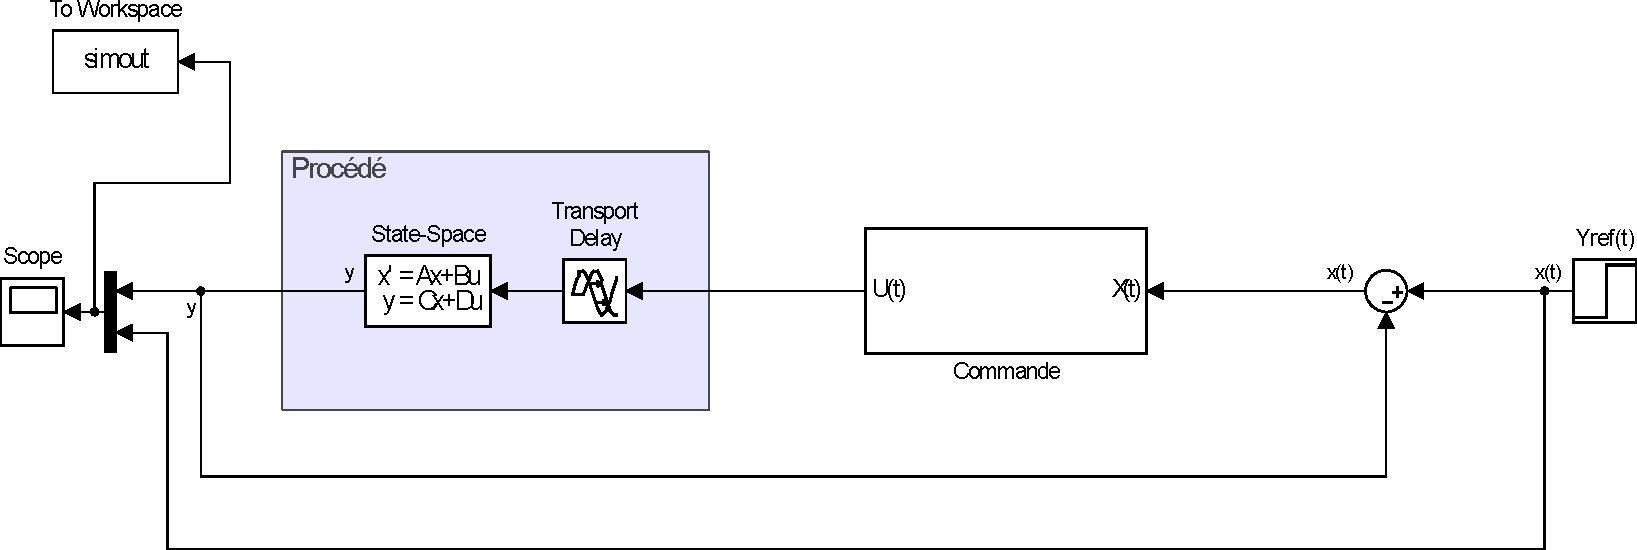
\includegraphics[width=\textwidth]{./III/images/sp1.pdf}
		\caption{\label{fig:sp1}Modèle SIMULINK du système en boucle fermé avec correcteur par retour d'état spectre fini (schéma général).}
	\end{minipage}\hfill
	\begin{minipage}{.48\textwidth}
		\centering
		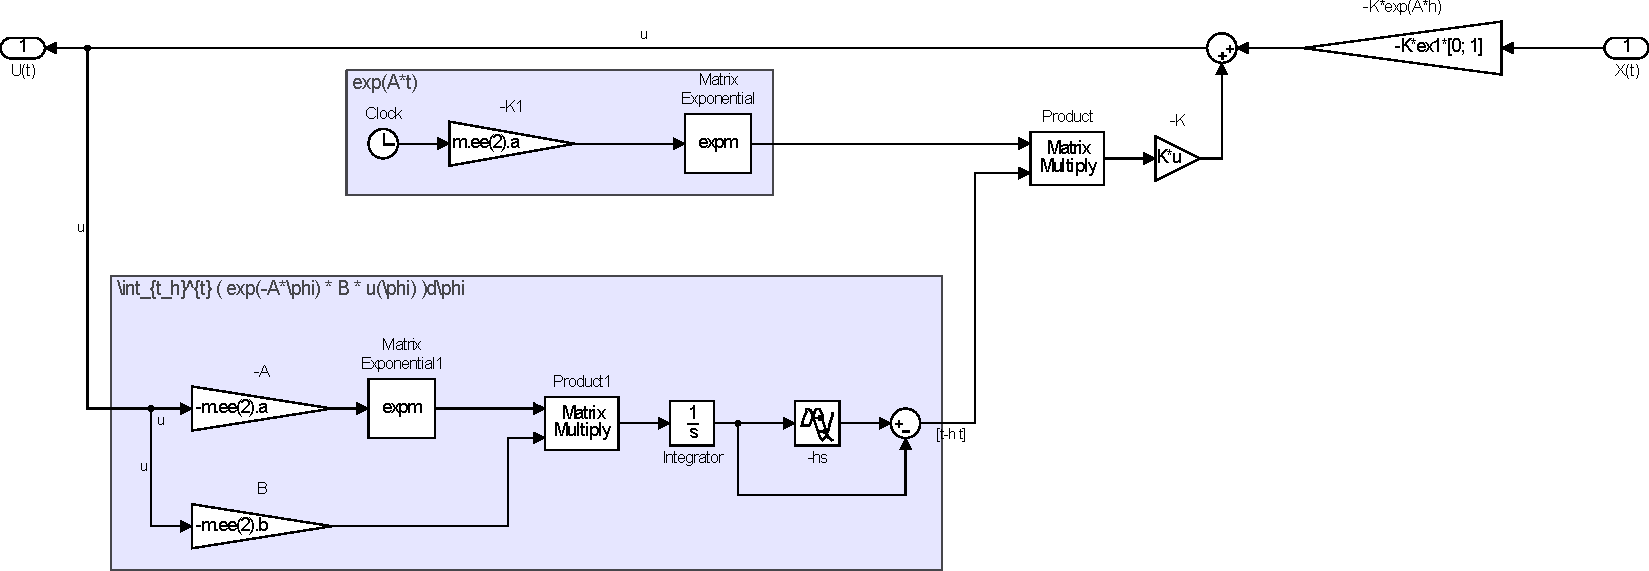
\includegraphics[width=\textwidth]{./III/images/sp2.pdf}
		\caption{\label{fig:sp2}Modèle SIMULINK du système en boucle fermé avec correcteur par retour d'état spectre fini (schéma bloc commande)}
	\end{minipage}
\end{figure}



\section{Robustesse de la commande}
Nous avons testé la commande sur une simulation de très longue durée (400s) et avec un solveur basé sur Euler, on s'aperçoit que le système diverge au bout d'un temps important de simulation ($\approx 300 s$). Cela est dû à l'intégration numérique qui transforme le système, sur un temps long, en un système neutre (voir figure \ref{fig:Vs400}.
\begin{figure}[!ht]
\centering
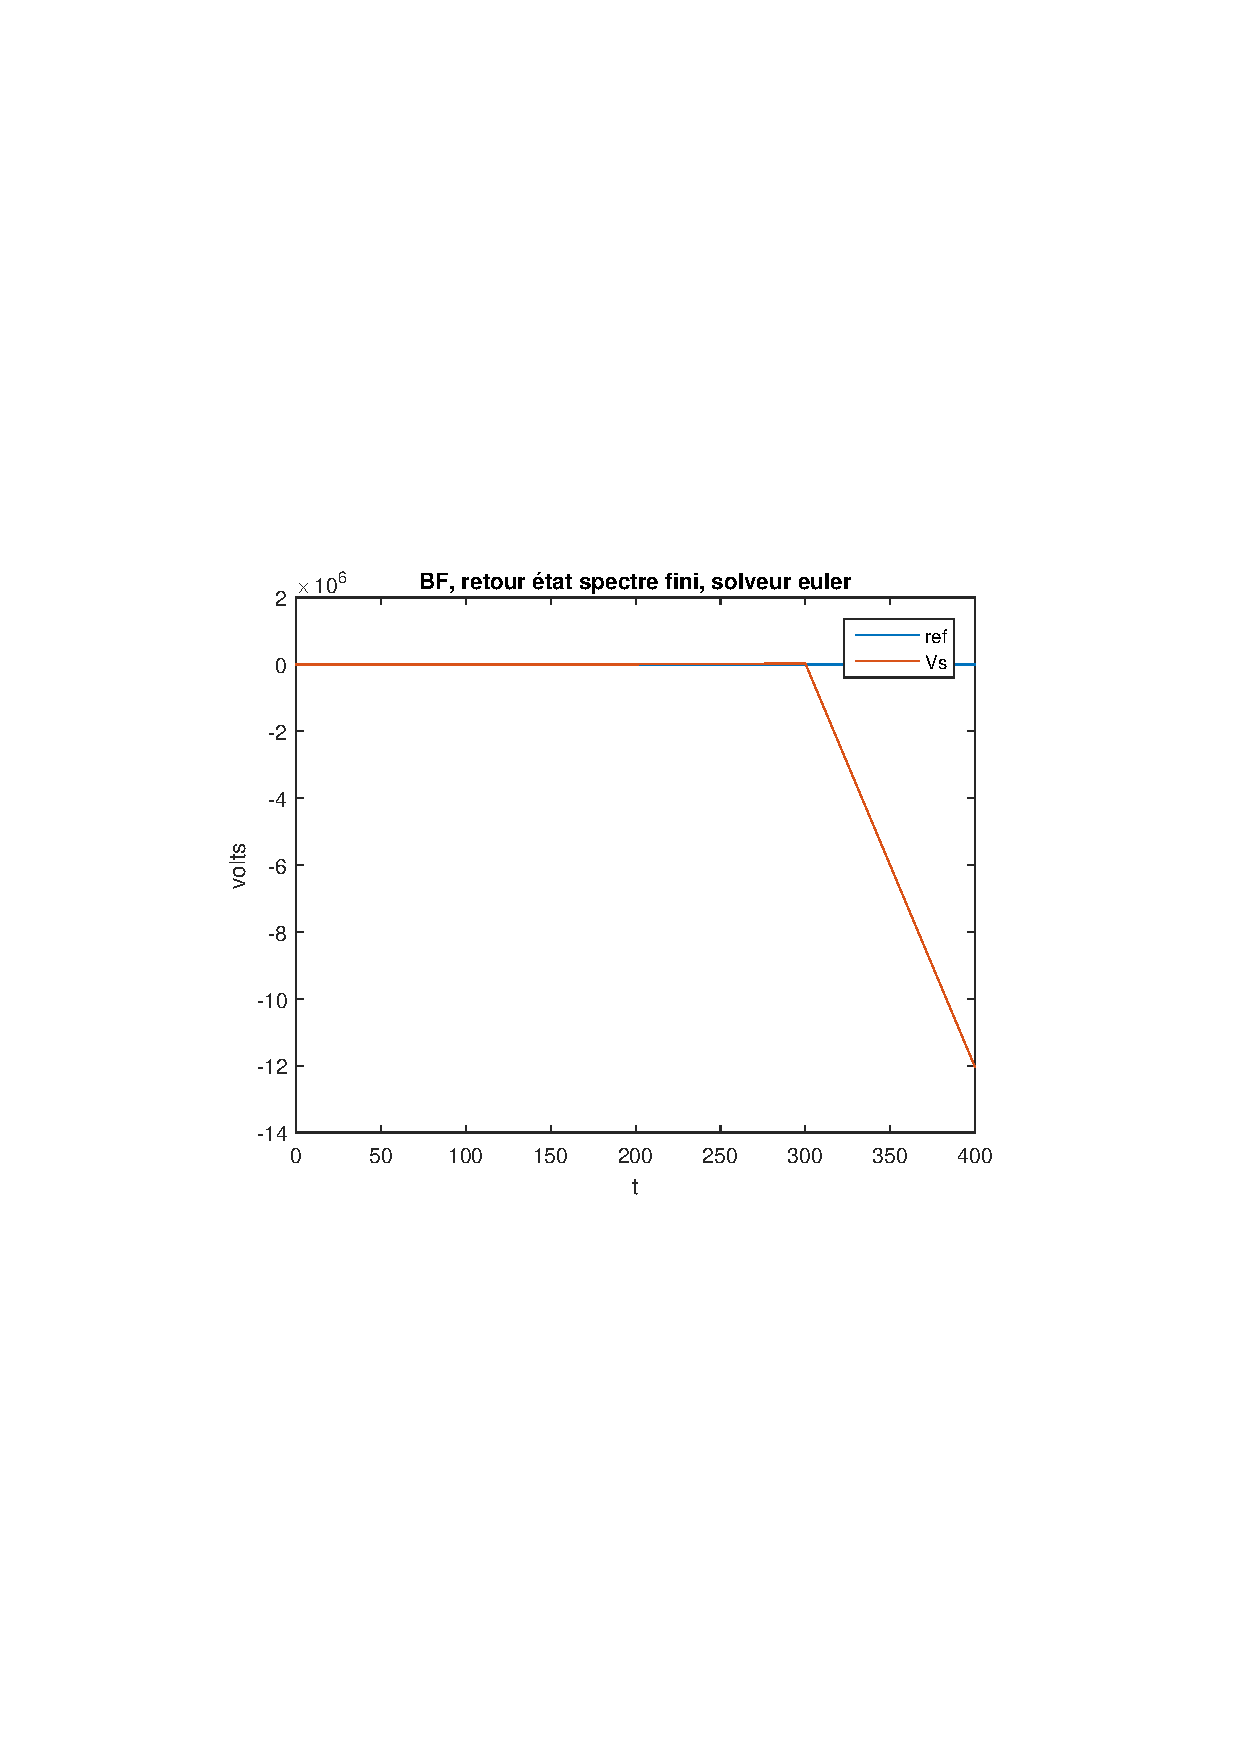
\includegraphics[width=.7\textwidth]{./III/images/Vg_RESpecFini_400.pdf}
\caption{\label{fig:Vs400} Réponse à un échelon unité de la différence des deux modèles.}
\end{figure}
